% Generated by code/needham.py -- do not edit by hand.
\definecolor{qocA}{rgb}{0.00,0.45,0.70}
\definecolor{qocB}{rgb}{0.90,0.60,0.00}
\definecolor{qocC}{rgb}{0.00,0.62,0.45}
\definecolor{qocD}{rgb}{0.80,0.40,0.00}
\definecolor{qocE}{rgb}{0.80,0.60,0.70}
\definecolor{qocF}{rgb}{0.35,0.70,0.90}
\begin{tikzpicture}[ink/.style={line width=0.9pt, ndInk}, faint/.style={line width=0.4pt, ndInk!35}, dashedink/.style={line width=0.5pt, ndInk!55, dash pattern=on 2.5pt off 2pt}, vec/.style={->, >=stealth, line width=1.2pt}, note/.style={font=\footnotesize\itshape, text=ndInk!85, align=center}, pointer/.style={->, >=stealth, line width=0.4pt, ndInk!60, shorten >=2pt, shorten <=1pt}, dot/.style={circle, fill=ndInk, inner sep=0pt, minimum size=3.4pt}, wash/.style={fill=ndSky, fill opacity=0.55}, every node/.style={text=ndInk}]
\definecolor{ndInk}{rgb}{0.13,0.13,0.18}
\definecolor{ndPaper}{rgb}{0.99,0.96,0.88}
\definecolor{ndSky}{rgb}{0.84,0.91,0.98}
\definecolor{ndRose}{rgb}{0.98,0.86,0.84}
\definecolor{ndBlue}{rgb}{0.13,0.36,0.66}
\definecolor{ndRed}{rgb}{0.78,0.20,0.16}
\definecolor{ndGold}{rgb}{0.88,0.62,0.10}
\definecolor{ndGreen}{rgb}{0.18,0.52,0.30}
\node[anchor=east] at (1.15,3.75) {$J(\Phi)\;=$};
\draw[ndInk, line width=0.9pt] (1.550,4.65) -- (1.550,3.000) arc (180:360:0.5) -- (2.550,3.48);
\node[rounded corners=3pt, draw=ndRed, fill=ndRose, line width=0.9pt, minimum size=0.55cm, inner sep=0pt, font=\scriptsize] (phi) at (2.550,3.75) {$\Phi$};
\draw[ndInk, line width=0.9pt] (phi.north) -- (2.550,4.65);
\node[font=\scriptsize, anchor=south] at (1.430,4.65) {reference};
\node[font=\scriptsize, anchor=south] at (2.650,4.65) {output};
\node[note, anchor=west] (cup) at (3.05,2.55) {the cup:\\ $\sum_i\ket{ii}$};
\draw[pointer] (cup.west) to[bend left=20] (2.170,2.520);
\node[font=\small] at (1.95,1.95) {CP $\iff J\succeq0$};
\node[rounded corners=3pt, draw=ndRed, fill=ndRose, line width=0.9pt, minimum size=0.55cm, inner sep=0pt, font=\scriptsize] (phi2) at (0.75,0.85) {$\Phi$};
\draw[ndInk, line width=0.9pt] (0.75,0.2) -- (phi2.south);
\draw[ndInk, line width=0.9pt] (phi2.north) -- (0.75,1.35);
\draw[ndInk, line width=0.9pt] (0.580,1.350) -- (0.920,1.350);
\draw[ndInk, line width=0.9pt] (0.640,1.420) -- (0.860,1.420);
\draw[ndInk, line width=0.9pt] (0.700,1.490) -- (0.800,1.490);
\node at (1.45,0.85) {$=$};
\draw[ndInk, line width=0.9pt] (2.05,0.2) -- (2.05,1.35);
\draw[ndInk, line width=0.9pt] (1.880,1.350) -- (2.220,1.350);
\draw[ndInk, line width=0.9pt] (1.940,1.420) -- (2.160,1.420);
\draw[ndInk, line width=0.9pt] (2.000,1.490) -- (2.100,1.490);
\node[note, anchor=west] at (2.45,0.85) {TP: discarding\\ after $\Phi$ is\\ discarding,\\ $\Tr_2J=\Id$};
\node[font=\small] at (2.1,-0.75) {(a) the Choi matrix};
\node[anchor=east] at (6.05,3.600) {$\Phi(\rho)\;=$};
\node[rounded corners=3pt, draw=ndRed, fill=ndRose, line width=0.9pt, minimum size=0.55cm, inner sep=0pt, font=\scriptsize] (V) at (6.750,3.600) {$V$};
\node[draw=ndGold!70!ndInk, fill=ndGold!25, rounded corners=3pt, line width=0.9pt, minimum size=0.5cm, inner sep=1pt, font=\scriptsize] (r) at (7.850,3.600) {$\rho$};
\node[rounded corners=3pt, draw=ndRed, fill=ndRose, line width=0.9pt, minimum size=0.55cm, inner sep=0pt, font=\scriptsize] (W) at (8.950,3.600) {$V^\dagger$};
\draw[ndInk, line width=0.9pt] (6.15,3.600) -- (V.west);
\draw[ndInk, line width=0.9pt] (V.east) -- (r.west);
\draw[ndInk, line width=0.9pt] (r.east) -- (W.west);
\draw[ndInk, line width=0.9pt] (W.east) -- (9.55,3.600);
\draw[ndGold!70!ndInk, line width=0.9pt] (V.north) -- (6.750,4.150) .. controls (6.750,5.000) and (8.950,5.000) .. (8.950,4.150) -- (W.north);
\node[font=\scriptsize, text=ndGold!70!ndInk, anchor=south] at (7.85,4.82) {environment $E$, discarded};
\node[font=\small] at (7.85,2.72) {$V=\sum_kK_k\otimes\ket k_E,\quad V^\dagger V=\Id$};
\node[anchor=east] at (6.05,1.100) {$\Phi(\rho)\;=$};
\node[rounded corners=3pt, draw=ndRed, fill=ndRose, line width=0.9pt, minimum size=0.55cm, inner sep=0pt, font=\scriptsize] (Vg) at (6.750,1.100) {$V$};
\node[draw=ndGold!70!ndInk, fill=ndGold!25, rounded corners=3pt, line width=0.9pt, minimum size=0.5cm, inner sep=1pt, font=\scriptsize] (rg) at (7.850,1.100) {$\rho$};
\node[rounded corners=3pt, draw=ndRed, fill=ndRose, line width=0.9pt, minimum size=0.55cm, inner sep=0pt, font=\scriptsize] (Wg) at (8.950,1.100) {$V^\dagger$};
\draw[ndInk, line width=0.9pt] (6.15,1.100) -- (Vg.west);
\draw[ndInk, line width=0.9pt] (Vg.east) -- (rg.west);
\draw[ndInk, line width=0.9pt] (rg.east) -- (Wg.west);
\draw[ndInk, line width=0.9pt] (Wg.east) -- (9.55,1.100);
\node[minimum size=0.34cm, inner sep=0pt, fill=ndGreen!20, draw=ndGreen, line width=0.9pt, font=\tiny] (u) at (6.750,1.720) {$u$};
\node[minimum size=0.34cm, inner sep=0pt, fill=ndGreen!20, draw=ndGreen, line width=0.9pt, font=\tiny] (ud) at (8.950,1.720) {$u^{\dagger}$};
\draw[ndGold!70!ndInk, line width=0.9pt] (Vg.north) -- (u.south);
\draw[ndGold!70!ndInk, line width=0.9pt] (Wg.north) -- (ud.south);
\draw[ndGold!70!ndInk, line width=0.9pt] (u.north) .. controls (6.750,2.600) and (8.950,2.600) .. (ud.north);
\node[note, anchor=north] at (7.85,0.52) {a unitary on the environment:\\ the Kraus operators $\sum_ku_{lk}K_k$\\ give the same $\Phi$};
\node[font=\small] at (7.85,-0.75) {(b) Stinespring and Kraus};
\draw[faint] (10.500,3.750) -- (12.060,3.750);
\fill[ndBlue!45, draw=ndBlue, line width=0.5pt] (10.700,3.750) rectangle (10.940,4.750);
\node[circle, fill=ndInk!40, inner sep=0pt, minimum size=1.6pt] at (11.180,3.750) {};
\node[circle, fill=ndInk!40, inner sep=0pt, minimum size=1.6pt] at (11.500,3.750) {};
\node[circle, fill=ndInk!40, inner sep=0pt, minimum size=1.6pt] at (11.820,3.750) {};
\node[font=\scriptsize, anchor=west, text=ndInk] at (12.030,4.030) {rank 1};
\node[font=\scriptsize, anchor=north west, inner sep=1pt] at (10.480,3.690) {unitary};
\draw[faint] (13.850,3.750) -- (15.410,3.750);
\fill[ndBlue!45, draw=ndBlue, line width=0.5pt] (14.050,3.750) rectangle (14.290,4.500);
\fill[ndBlue!45, draw=ndBlue, line width=0.5pt] (14.370,3.750) rectangle (14.610,4.000);
\node[circle, fill=ndInk!40, inner sep=0pt, minimum size=1.6pt] at (14.850,3.750) {};
\node[circle, fill=ndInk!40, inner sep=0pt, minimum size=1.6pt] at (15.170,3.750) {};
\node[font=\scriptsize, anchor=west, text=ndInk] at (15.380,4.030) {rank 2};
\node[font=\scriptsize, anchor=north west, inner sep=1pt] at (13.830,3.690) {amplitude damping, $\gamma=0.5$};
\draw[faint] (10.500,2.150) -- (12.060,2.150);
\fill[ndBlue!45, draw=ndBlue, line width=0.5pt] (10.700,2.150) rectangle (10.940,2.950);
\fill[ndBlue!45, draw=ndBlue, line width=0.5pt] (11.020,2.150) rectangle (11.260,2.350);
\node[circle, fill=ndInk!40, inner sep=0pt, minimum size=1.6pt] at (11.500,2.150) {};
\node[circle, fill=ndInk!40, inner sep=0pt, minimum size=1.6pt] at (11.820,2.150) {};
\node[font=\scriptsize, anchor=west, text=ndInk] at (12.030,2.430) {rank 2};
\node[font=\scriptsize, anchor=north west, inner sep=1pt] at (10.480,2.090) {dephasing, $p=0.2$};
\draw[faint] (13.850,2.150) -- (15.410,2.150);
\fill[ndBlue!45, draw=ndBlue, line width=0.5pt] (14.050,2.150) rectangle (14.290,2.775);
\fill[ndBlue!45, draw=ndBlue, line width=0.5pt] (14.370,2.150) rectangle (14.610,2.275);
\fill[ndBlue!45, draw=ndBlue, line width=0.5pt] (14.690,2.150) rectangle (14.930,2.275);
\fill[ndBlue!45, draw=ndBlue, line width=0.5pt] (15.010,2.150) rectangle (15.250,2.275);
\node[font=\scriptsize, anchor=west, text=ndInk] at (15.380,2.430) {rank 4};
\node[font=\scriptsize, anchor=north west, inner sep=1pt] at (13.830,2.090) {depolarising, $\lambda=0.5$};
\draw[faint] (10.500,0.550) -- (12.060,0.550);
\fill[ndBlue!45, draw=ndBlue, line width=0.5pt] (10.700,0.550) rectangle (10.940,1.311);
\fill[ndBlue!45, draw=ndBlue, line width=0.5pt] (11.020,0.550) rectangle (11.260,0.698);
\fill[ndBlue!45, draw=ndBlue, line width=0.5pt] (11.340,0.550) rectangle (11.580,0.641);
\node[circle, fill=ndInk!40, inner sep=0pt, minimum size=1.6pt] at (11.820,0.550) {};
\node[font=\scriptsize, anchor=west, text=ndInk] at (12.030,0.830) {rank 3};
\node[font=\scriptsize, anchor=north west, inner sep=1pt] at (10.480,0.490) {the damped qubit, $t=1$};
\draw[faint] (13.850,0.550) -- (15.410,0.550);
\fill[ndBlue!45, draw=ndBlue, line width=0.5pt] (14.050,0.550) rectangle (14.290,1.050);
\fill[ndBlue!45, draw=ndBlue, line width=0.5pt] (14.370,0.550) rectangle (14.610,1.050);
\fill[ndBlue!45, draw=ndBlue, line width=0.5pt] (14.690,0.550) rectangle (14.930,1.050);
\fill[ndRed!45, draw=ndRed, line width=0.5pt] (15.010,0.550) rectangle (15.250,0.050);
\node[font=\scriptsize, anchor=west, text=ndRed] at (15.380,0.830) {not CP: $-\tfrac12$};
\node[font=\scriptsize, anchor=north west, inner sep=1pt] at (13.830,-0.010) {transposition};
\node[font=\small] at (13.75,-0.75) {(c) the eigenvalues of $J/N$: the Kraus rank};
\end{tikzpicture}
